\documentclass[tikz,border=12pt]{standalone}
% Shared visual language for standalone EMT block diagrams.
\usepackage{amsmath}
\usetikzlibrary{arrows.meta,backgrounds,calc,fit,positioning}

\tikzset{
    emt diagram/.style = {>={Stealth[length=2.4mm]}},
    line/.style        = {semithick, rounded corners=6pt},
    block/.style       = {draw, semithick, fill=white,
                          minimum height=1cm, minimum width=2.3cm},
    hblock/.style      = {block, minimum width=2.24cm, minimum height=1.3cm},
    vblock/.style      = {block, minimum width=1.3cm, minimum height=2.24cm},
    sum/.style         = {draw, semithick, fill=white, circle,
                          inner sep=2.6pt},
    signal/.style      = {circle, fill, inner sep=1.4pt,
                          label distance=3pt},
    sig/.style         = {font=\small},
    pm/.style          = {font=\scriptsize},
    wire jump/.style   = {line,
                          preaction={draw=white, line width=3pt,
                                     line cap=round}},
    enclosure/.style   = {draw, dashed, semithick, rounded corners=4pt},
    operator enclosure/.style = {enclosure, inner xsep=7mm, inner ysep=6mm}
}


\begin{document}
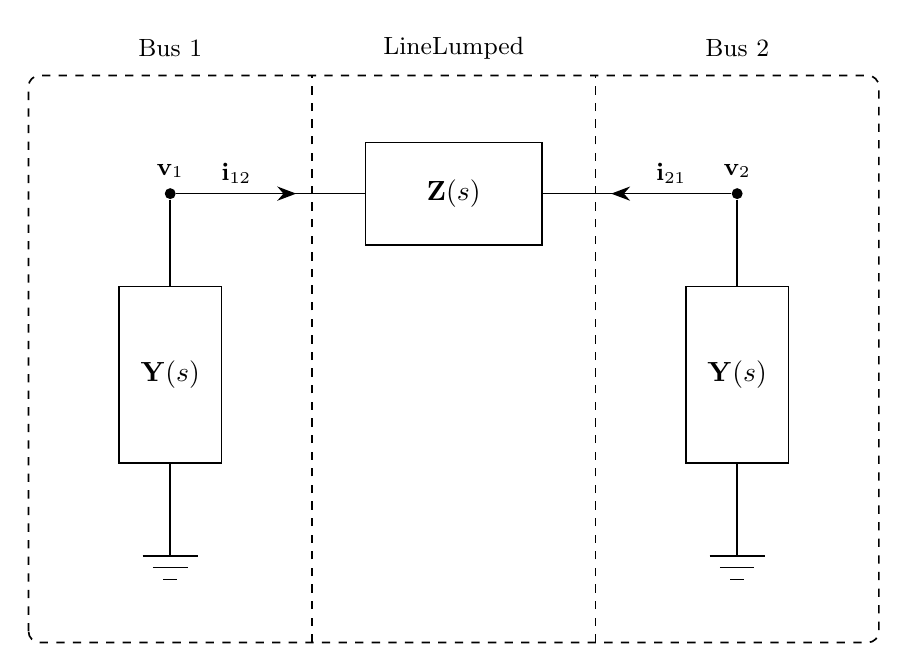
\begin{tikzpicture}[emt diagram]

% ================= Series branch Z(s) =================
\node[hblock] (Z) at (0, 2.1) {$\mathbf{Z}(s)$};

% ================= Shunt branches Y(s) =================
\node[vblock] (Yk) at (-3.6, -0.2) {$\mathbf{Y}(s)$};
\node[vblock] (Ym) at ( 3.6, -0.2) {$\mathbf{Y}(s)$};

% ================= Voltage terminals =================
\node[signal, label={[sig]above:$\mathbf{v}_1$}] (Tk) at (-3.6, 2.1) {};
\node[signal, label={[sig]above:$\mathbf{v}_2$}] (Tm) at ( 3.6, 2.1) {};

% ================= Series terminal currents =================
\draw[line] (Z.west) -- (Tk);
\draw[line] (Z.east) -- (Tm);
\draw[->, line] (Tk) -- (-2.0,2.1)
    node[midway, above, sig] {$\mathbf{i}_{12}$};
\draw[->, line] (Tm) -- (2.0,2.1)
    node[midway, above, sig] {$\mathbf{i}_{21}$};

% ================= Shunt wiring =================
\draw[line] (Tk) -- (Yk.north);
\draw[line] (Tm) -- (Ym.north);
\draw[line] (Yk.south) -- (-3.6, -2.5);
\draw[line] (Ym.south) -- ( 3.6, -2.5);

% ================= Ground symbols =================
\draw[semithick] (-3.95,-2.50) -- (-3.25,-2.50);
\draw[semithick] (-3.82,-2.65) -- (-3.38,-2.65);
\draw[semithick] (-3.69,-2.80) -- (-3.51,-2.80);

\draw[semithick] ( 3.25,-2.50) -- ( 3.95,-2.50);
\draw[semithick] ( 3.38,-2.65) -- ( 3.82,-2.65);
\draw[semithick] ( 3.51,-2.80) -- ( 3.69,-2.80);

% ================= Ownership =================
\draw[enclosure] (-5.4, -3.6) rectangle (5.4, 3.6);
\draw[dashed, semithick] (-1.8, -3.6) -- (-1.8, 3.6);
\draw[dashed, semithick] ( 1.8, -3.6) -- ( 1.8, 3.6);
\node[sig] at (-3.6,3.95) {Bus 1};
\node[sig] at (0,3.95) {LineLumped};
\node[sig] at (3.6,3.95) {Bus 2};

\end{tikzpicture}
\end{document}
